

\title{Laboratorium 2 - Sprawozdanie}
\author{Wojciech Makuch}

	\maketitle
	\section{Zadanie}
	Program framework benchmarkujacy dla zaimpleentowanych struktur Stos, Lista, Kolejka.
	\section{Realizacja}
	Program zawiera 3 struktury danych. Każda z nich zawiera 3 podstawowe metody: połóż element, zdejmij element, zwróć rozmiar. Struktua Stos zbudowana za pomocą tablicy z realokacją pamięci, Lista ze wskaźnikiem na następny element, oraz Kolejka z indeksami na pierwszy i ostatni element. Wszystki struktury danych działają prawidłowo.
	Ponadto program zawiera fnkcje wypęłniającą struktury liczbami psełdolosowymi oraz zliczającą czas dla przeprowadzenia testów złożonosci obliczeniowej ww struktur.
	\section{Działanie}
	Głowna funkcja programu kolejno tworzy struktury Stos, Lista, Koljaka(a po zakończeniu operacji na nich, zwalnia pamięć), następnie za pomącą funkcji zliczającej czas wykonuje testy złożonosci obliczeniowej. Uzyskae wyniki program wyświetla na ekranie oray zapisuje do pliku o nazwie \textsl{Pomiar\_czasu2.txt.}
	\section{Wyniki}
	Najszybsze działanie algorytmu wypęłniania struktur liczbami pesęłdolosowymi wykonuje lista, następnie Kolajka, a na samym konsu Stos. Lista ponadto może pomieścić najwięcej elementów, najniej - Kolejka. Na wykresie w skali logarytmicznej pokazano zależność wykonanym operacji do czasu. Widać, że krzywe mozna przybliżyć prostymi, z czego wniosek, że złożoność obliczeniowa wynosi O(n).  
	 \begin{figure}
	 	\centering
		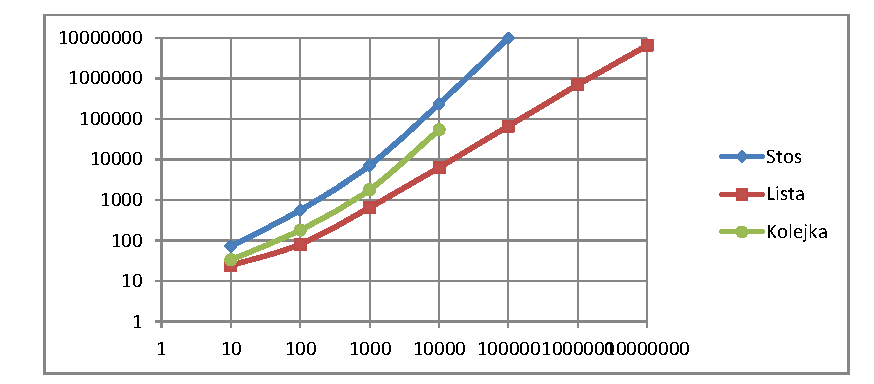
\includegraphics[width=14cm]{Wykres.pdf}
		\caption{Wykres złożoności obliczeniowej.}
	 \end{figure}
	 \section{Komentarz}
	 	Do utworzenia dokumentacji wykorzystano system Doxygen.
	 	Funkcja pomiaru czasu dla systemu Windows pobrana ze strony dr. J. Mierzwy. Program skompilowano w środowisku Code::Blocks. Do stworzonia wykresu posłużono się pakietem MS Excel, sprawozdanie napisano uzywając systemu \LaTeX.
\end{document}